\documentclass{article} % PDFTex, XeLaTex 都支持。

% 中文环境
%\documentclass[hyperref, UTF8]{ctexart} %若选择{ctexart}则直接支持中文,下面的{ctex}要去掉。
\usepackage[UTF8]{ctex} %中文配置。
%\usepackage[UTF8, heading=false, scheme=plain]{ctex} %加入scheme=plain,行距、中西文公共字符都有变化。

% 版面设置
\usepackage{geometry}
\geometry{a4paper}

% 额外的功能
\usepackage{authblk} %添加机构,需要安装preprint包
\usepackage{amsthm} %证明环境
\usepackage{amsmath} %数学公式
\numberwithin{equation}{section} % 公式按章节编号
\usepackage{amssymb}
\usepackage{multirow} % multirow
\usepackage{booktabs} % toprule, midrule, bottomrule

% 表格的单元格内换行、对齐功能
\usepackage{makecell}

% 图片支持
\usepackage{graphicx} %添加图片
\graphicspath{{figures/}}
\usepackage{float} % 控制图片是否浮动:[htbp]浮动,或[H]禁止浮动

% PDF索引及超链接 (black,red,blue,green)
\usepackage[colorlinks=true,linkcolor=black,anchorcolor=black,citecolor=blue,filecolor=black,menucolor=black,runcolor=black,urlcolor=black]{hyperref}

% 首行缩进
\usepackage{indentfirst} % 首行缩进支持
\setlength{\parindent}{2em} % 首行缩进两个汉字

% 列表样式定制
\usepackage{enumerate}
\usepackage{enumitem}
\setlist[enumerate,1]{label=(\arabic*).,font=\textup,leftmargin=14mm,labelsep=1.5mm,topsep=0mm,itemsep=-0.8mm}
\setlist[enumerate,2]{label=(\alph*).,font=\textup,leftmargin=14mm,labelsep=1.5mm,topsep=-0.8mm,itemsep=-0.8mm}
%\setlist{nosep} % 取消行间空行

% 自定义命令
\newcommand{\SL}{\rule{.3em}{.3pt}} % 定义短下划线

% 名称、作者、机构
\title{Formal Method Library \\for Altitude Representation System of FCS}
\author{Zhengpu Shi}
\affil{Draft V1.0}
%\affil{南京航空航天大学}
%\date{2020年12月29日} %注释后显示为编译时日期


\begin{document}

% 生成标题
\maketitle
\newpage
% ++++++++++++++++++++++++++++++++++++++++++++++++++++++++++++++++++++++++++++++++++++++++++++++++++

% 生成目录
\tableofcontents
\newpage
% ++++++++++++++++++++++++++++++++++++++++++++++++++++++++++++++++++++++++++++++++++++++++++++++++++

%\listoffigures
%\newpage
% 生成图片列表,请删除上面两行注释

%\begin{figure}[H]%[htbp]
%\centering
%\includegraphics[scale=0.6]{gradient.jpg}
%\caption{this is a figure demo}
%\label{fig:label}
%\end{figure}

\section{Introduction}
This is one part of the FML4FCS project. 
For detail information, please refer the introduction of the whole project in this website.


\newpage
% ++++++++++++++++++++++++++++++++++++++++++++++++++++++++++++++++++++++++++++++++++++++++++++++++++

\section{Attitude Representation System (ARS)}

In order to describe the attitude and position of the aircraft, we need to establish an appropriate coordinate system.
There are three main attitude representation methods of aircraft, including Euler Angle, rotation matrix and quaternion.
The mathematics we need include real numbers, vectors, matrices, quaternions, and so on.
Regarding Real numbers, there are two forms of Real number libraries included in COQ, ``Real'' and ``Float''.
The former is axiomatic realization, easy to prove; The latter is mapped to the concrete implementation, more intuitive.
Vectors, matrices, and quaternions are not available in libraries; we need to customize them.


% ----------------------------------------------------------------------------------------
\subsection{Derivation of the rotation matrix}

\subsubsection{Counterclockwise rotation of a 2D vector}

\begin{figure}[htbp]
\centering
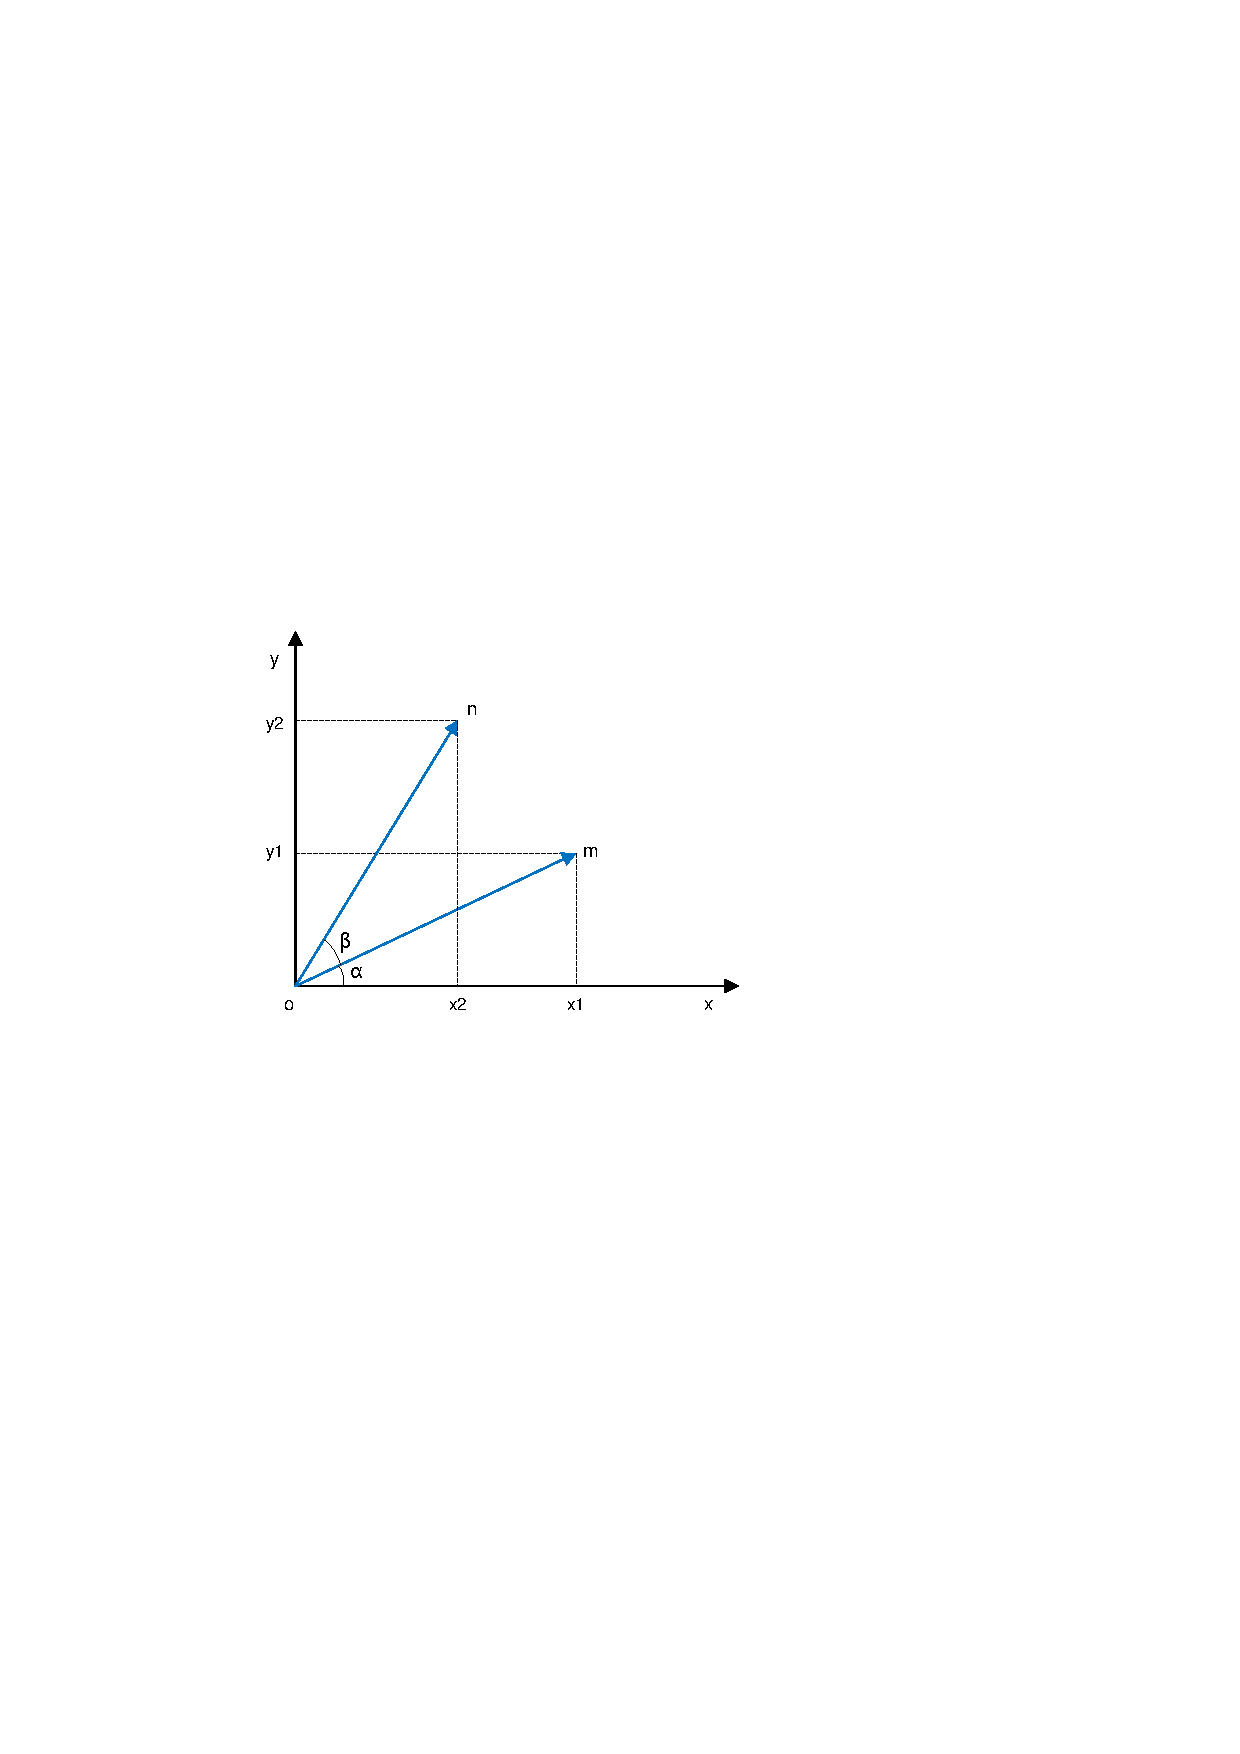
\includegraphics[width=0.40\textwidth]{derive_2d_rotation_matrix_anticlockwise.pdf}
\caption{2D Rotation Anticlockwise}
%\label{fig:label}
\end{figure}

Known: Give a vector $\overrightarrow{om}=[x1\quad y1]^T$, rotate it countclockwise by original point $\beta$ degree, 
then got $\overrightarrow{on}=[x2\quad y2]^T$。

Question: get transformation matrix $A(\beta)$ and $B(\beta)$ that could representation vector counterclockwise rotation by angle $\beta$ between $[x1\quad y1]^T$ and $[x2\quad y2]^T$ as follows.
\begin{equation}
\begin{bmatrix}x2\\y2\end{bmatrix}=A(\beta)\begin{bmatrix}x1\\y1\end{bmatrix}
\end{equation}

\begin{equation}
\begin{bmatrix}x1\\y1\end{bmatrix}=B(\beta)\begin{bmatrix}x2\\y2\end{bmatrix}
\end{equation}

Calculate:
\begin{enumerate}

\item Let the length of $\overrightarrow{om}$ is $l$, 
let the angle between $\overrightarrow{om}$ and $\overrightarrow{ox}$ is $\alpha$,
then the length of $\overrightarrow{on}$ is $l$, 
and the angle between $\overrightarrow{on}$ and $\overrightarrow{ox}$ is $\alpha+\beta$.
Then,
\begin{equation*}
\left\{\begin{array}{rl}
x1 &= l~\cos\alpha\\
y1 &= l~\sin\alpha\\
x2 &= l~\cos{(\alpha+\beta)}\\
y2 &= l~\sin{(\alpha+\beta)}
\end{array}\right.
\end{equation*}

\item Use the following trigonometric relationship
\begin{equation*}
\left\{\begin{array}{rl}
\sin{(\alpha+\beta)}& = \sin\alpha~\cos\beta + \cos\alpha~\sin\beta\\
\cos{(\alpha+\beta)}& = \cos\alpha~\cos\beta - \sin\alpha~\sin\beta
\end{array}\right.
\end{equation*}

\item Simplify and transform.
\begin{equation}\label{2d_rotation_matrix_anticlockwise_eq3}
\left\{\begin{array}{rl}
x2 &= \cos\beta~x1 - \sin\beta~y1\\
y2 &= \sin\beta~x1 + \cos\beta~y1
\end{array}\right.
\end{equation}

\item Transform
\begin{equation*}
\begin{bmatrix}x_2\\y_2\end{bmatrix}=
\begin{bmatrix}cos\beta & -sin\beta \\sin\beta & cos\beta \end{bmatrix}
\begin{bmatrix}x_1\\y_1\end{bmatrix}
\end{equation*}

\item Got matrix A
\begin{equation}\label{2d_rotation_matrix_anticlockwise_old_to_new}
A(\beta)=\begin{bmatrix}cos\beta & -sin\beta \\sin\beta & cos\beta \end{bmatrix}
\end{equation}

\item There are two methods to solve matrix B: 
first, using the derivation method above, second, get invert matrix of matrix A.
We use first method.
Left multiply $\cos\beta$ or $\sin\beta$ to the two equation of \eqref{2d_rotation_matrix_anticlockwise_eq3}, then:
\begin{equation}\label{2d_rotation_matrix_anticlockwise_eq4}
\left\{\begin{array}{rl}
\cos\beta~x2 &= \cos^2\beta~x1 - \sin\beta~\cos\beta~y1\\
\cos\beta~y2 &= \sin\beta~\cos\beta~x1 + \cos^2\beta~y1\\
\sin\beta~x2 &= \sin\beta~\cos\beta~x1 - \sin^2\beta~y1\\
\sin\beta~y2 &= \sin^2\beta~x1 + \sin\beta~\cos\beta~y1
\end{array}\right.
\end{equation}

\item Transform and get
\begin{equation}\label{2d_rotation_matrix_anticlockwise_eq6}
\left\{\begin{array}{rl}
x1 &= \cos\beta~x2 + \sin\beta~y2\\
y1 &= -\sin\beta~x2 + \cos\beta~y2
\end{array}\right.
\end{equation}

\item Write to matrix form
\begin{equation*}
\begin{bmatrix}x_1\\y_1\end{bmatrix}=
\begin{bmatrix}\cos\beta & \sin\beta \\-\sin\beta & \cos\beta \end{bmatrix}
\begin{bmatrix}x_2\\y_2\end{bmatrix}
\end{equation*}

\item Got matrix B
\begin{equation}\label{2d_rotation_matrix_anticlockwise_new_to_old}
B(\beta)=\begin{bmatrix}\cos\beta & \sin\beta \\-\sin\beta & \cos\beta \end{bmatrix}
\end{equation}

\end{enumerate}

\subsubsection{Clockwise rotation of a 2D vector}

\begin{figure}[htbp]
\centering
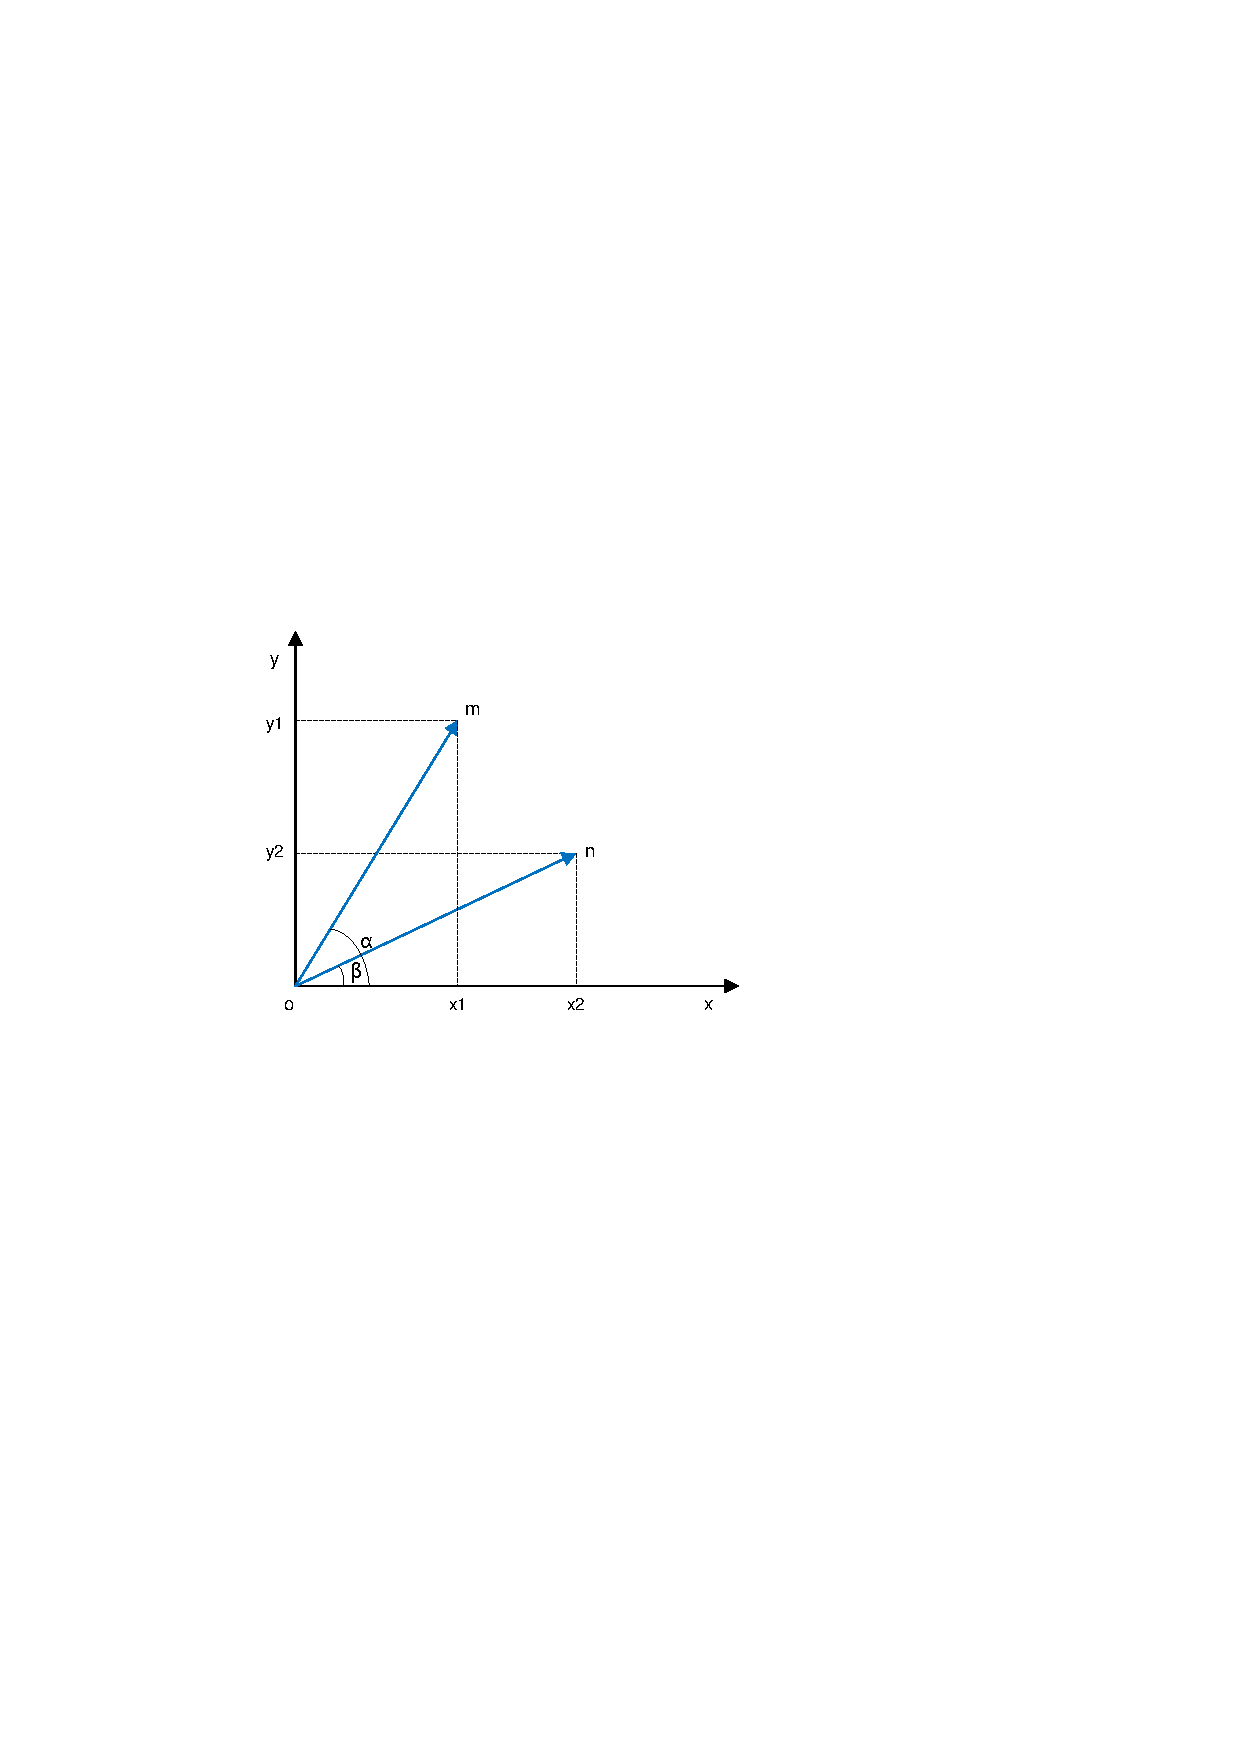
\includegraphics[width=0.40\textwidth]{derive_2d_rotation_matrix_clockwise.pdf}
\caption{2D Rotation Clockwise}
%\label{fig:label}
\end{figure}

Known: Give a vector$\overrightarrow{om}=[x1\quad y1]^T$, rotate it clockwise by original point $\beta$ degree, then got $\overrightarrow{on}=[x2\quad y2]^T$。

Question: get transformation matrix $C(\beta)$ and $D(\beta)$ that could representation vector clockwise rotation by angle $\beta$ between  $[x1\quad y1]^T$ and $[x2\quad y2]^T$ as follows.
\begin{equation}
\begin{bmatrix}x2\\y2\end{bmatrix}=C(\beta)\begin{bmatrix}x1\\y1\end{bmatrix}
\end{equation}

\begin{equation}
\begin{bmatrix}x1\\y1\end{bmatrix}=D(\beta)\begin{bmatrix}x2\\y2\end{bmatrix}
\end{equation}

Calculate:
It's easy to get the answer in the same way shown above.
\begin{equation}\label{2d_rotation_matrix_clockwise_new_to_old}
C(\beta)=\begin{bmatrix}\cos\beta & \sin\beta \\-\sin\beta & \cos\beta \end{bmatrix}
\end{equation}

\begin{equation}\label{2d_rotation_matrix_clockwise_old_to_new}
D(\beta)=\begin{bmatrix}\cos\beta & -\sin\beta \\ \sin\beta & \cos\beta \end{bmatrix}
\end{equation}

In fact, we find that $A(\beta)$ and $B(\beta)$ are inverse matrices, and $A(\beta)=D(\beta), B(\beta)=C(\beta)$。
These are the only two kinds of matrices that occur when you rotate in 2D coordinates.

In fact, the representation of the vector before rotation and the vector after rotation is a inverse operation. 
And clockwise and counterclockwise rotation are also inverse operations.
That's why we could get a pair of inverse matrix.

\begin{equation}\label{2d_rotation_matrix_anticlockwise_old_to_new}
\begin{bmatrix}\cos\beta & -\sin\beta \\ \sin\beta & \cos\beta \end{bmatrix}
\begin{bmatrix}\cos\beta & \sin\beta \\-\sin\beta & \cos\beta \end{bmatrix} =
\begin{bmatrix}1&0\\0&1\end{bmatrix}
\end{equation}

\begin{equation}\label{2d_rotation_matrix_anticlockwise_old_to_new}
\begin{bmatrix}\cos\beta & -\sin\beta \\ \sin\beta & \cos\beta \end{bmatrix} = 
\begin{bmatrix}\cos\beta & \sin\beta \\-\sin\beta & \cos\beta \end{bmatrix}^{-1}
\end{equation}

And by the way, this is a derivation of rotations in the real field, which is much simpler if you do it in complex numbers.

\subsubsection{Basic rotation of a vector about the coordinate axis in 3D}

So if you rotate a vector in three dimensions around some axis, you just keep the coordinates of the components of the axis of rotation the same, and then you just do the two axes in 2D.

You need to specify whether the rotation direction is clockwise or counterclockwise, and along which direction to look.

The direction of observation is not emphasized in the 2D rotation, if you are looking at our rotation diagram on the computer screen, the direction of observation is looking at the screen.
But 3D is especially important, because it's easy to get it wrong.

We skip the derivation and give a rotation matrix about the $x,y,z$ axes, all in the positive direction, as defined in \ref{right_hand_rule}.

The basic rotation matrix that rotates the vector in the positive direction.
\begin{equation}\label{3d_rotation_matrix_rot_vec}
	\left\{
		\begin{array}{rl}
			R_x(\alpha)\vspace{1ex} &=\begin{bmatrix}
				1 & 0 & 0\\
				0 & \cos\alpha & -sin\alpha\\
				0 & \sin\alpha & cos\alpha
			\end{bmatrix}\\
			R_y(\beta)\vspace{1ex} &=\begin{bmatrix}
				\cos\beta & 0 & -\sin\beta\\
				0 & 1 & 0\\
				\sin\beta & 0 & \cos\beta
			\end{bmatrix}\\
			R_z(\gamma) &=\begin{bmatrix}
				\cos\gamma & -\sin\gamma & 1\\
				\sin\gamma & \cos\gamma & 1\\
				0 & 0 & 1
			\end{bmatrix}
		\end{array}
	\right.
\end{equation}

An example is given to illustrate how to use it.

For example, (positive) rotate vector $om=[x1\quad y1\quad z1]^T$ by $\alpha$ degree about $x$ axis, then we get $on=[x2\quad y2\quad z2]^T$.
\begin{figure}[htbp]
\centering
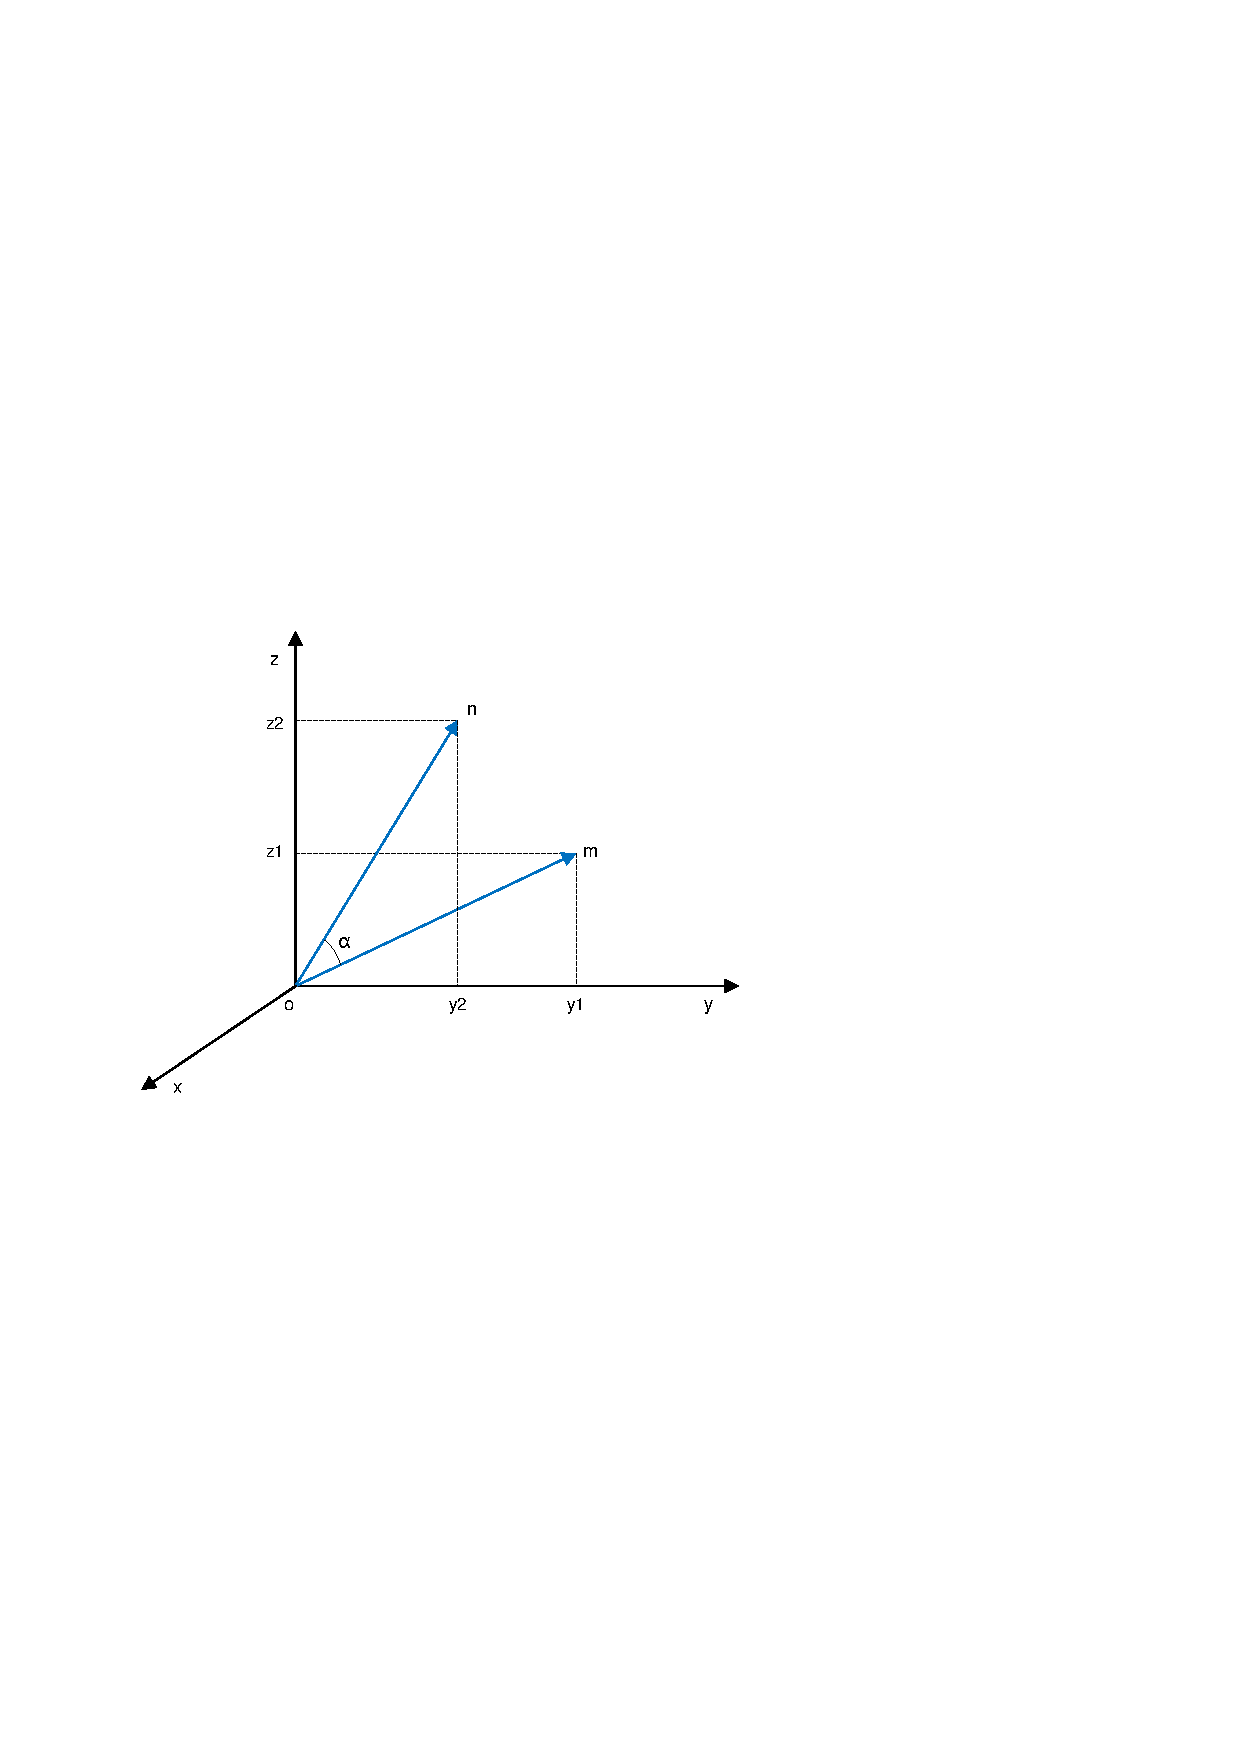
\includegraphics[width=0.50\textwidth]{derive_3d_rotation_matrix_rotate_x.pdf}
\caption{3D Rotation by X Axis}
%\label{fig:label}
\end{figure}

\begin{equation}
\begin{bmatrix}x2\\y2\\z2\end{bmatrix}=R_x(\alpha)\begin{bmatrix}x1\\y1\\z1\end{bmatrix}
\end{equation}

\subsubsection{Basic rotation of coordinate along an axis in 3D}
The basic rotation matrices for rotation of coordinate along an axis in 3D are belows.
\begin{equation}\label{3d_rotation_matrix_rot_axis}
	\left\{
		\begin{array}{rl}
			R_x(\alpha)^{'}\vspace{1ex} &=\begin{bmatrix}
				1 & 0 & 0\\
				0 & \cos\alpha & \sin\alpha\\
				0 & -\sin\alpha & \cos\alpha
			\end{bmatrix}\\
			R_y(\beta)^{'}\vspace{1ex} &=\begin{bmatrix}
				\cos\beta & 0 & \sin\beta\\
				0 & 1 & 0\\
				-\sin\beta & 0 & \cos\beta
			\end{bmatrix}\\
			R_z(\gamma)^{'} &=\begin{bmatrix}
				\cos\gamma & \sin\gamma & 1\\
				-\sin\gamma & \cos\gamma & 1\\
				0 & 0 & 1
			\end{bmatrix}
		\end{array}
	\right.
\end{equation}

\subsubsection{The relationship between vector rotatation and coordinate rotation}

The vector rotation operation is only for a given vector.
The coordinate rotation operation is for all the vectors.
By the way, vector rotation and coordinate rotation are inverse operations each other.

We have two choices of rotation direction (positive and negative) and three choices of coordinate axes ($x,y,z$), so we have $2\times 3=6$ different matrices ($R_x(\alpha),$ $R_y(\beta),$ $R_z(\gamma),$ $R_x(\alpha)^{'},$ $R_y(\beta)^{'},$ $R_z(\gamma)^{'}$) to handle 3D rotations.
These 6 rotation matrices all are $SO3$ matrices, and any finite times composition of them are $SO3$ matrices too.

$SO3$ matrices should satisfy: transposed matrix is itself, the determinant of the matrix is 1.

% ----------------------------------------------------------------------------------------
\subsection{Coordinate System}

\subsubsection{Right-Hand Rule}\label{right_hand_rule}

\begin{figure}[htbp]
\centering
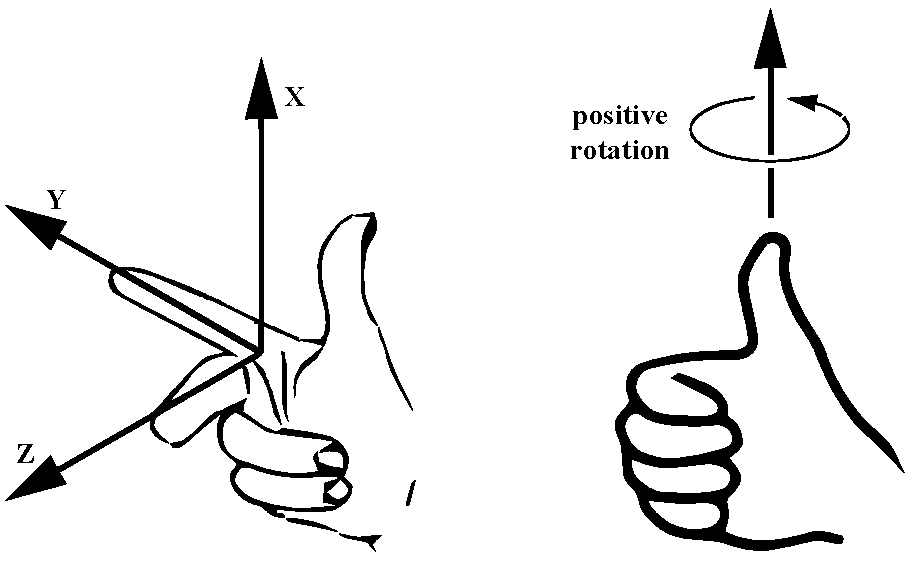
\includegraphics[width=0.50\textwidth]{right_hand_rule.pdf}
\caption{Right hand rule}
\label{fig:right_hand_rule}
\end{figure}

The right-hand rule determines the positive direction of the three axes of a 3D coordinate system.
As shown in \ref{fig:right_hand_rule}, extend the thumb, index finger and middle finger of the right hand vertically, the intersection of the three fingers represents the origin of coordinates, the outward directions of the thumb, index finger and middle finger are respectively the positive directions of the ox, oy and oz axes.
The right hand-rule can also determine the positive direction of the rotation angle when rotating about an axis.
To do this, straighten the thumb of your right hand and point in the same positive direction as the axis of rotation. Bend four fingers and mark the direction of the stroke as the positive direction of rotation.

\subsubsection{Earth Fixed Coordinate Frame(EFCF)}
\begin{figure}[htbp]
\centering
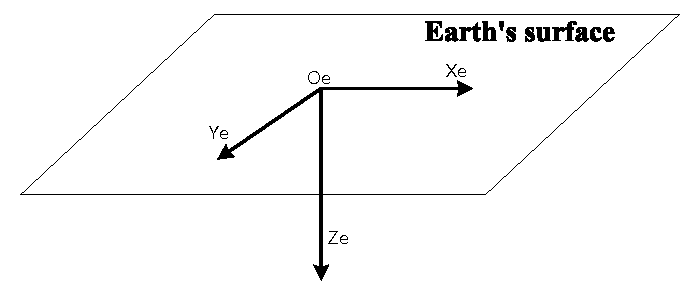
\includegraphics[width=0.50\textwidth]{earth_surface_coordinate.pdf}
\caption{Earth Fixed Coordinate Frame}
%\label{fig:label}
\end{figure}

地球固连坐标系,也称作导航参考坐标系。
这个坐标系不会移动,并且已附加到地球的局部切线平面上。
当地面上的飞机起飞时,将飞机质心的位置当做EFCF的原点$o_e$,
以垂直于地面向下作为$o_e z_e$轴正向,在水平面内任取某一方向为$o_e x_e$正方向,然后用右手定则确定$o_e y_e$正方向。
一般的,导航坐标系被当做是牛顿定理适用的局部惯性坐标系。

\subsubsection{机体坐标系}
\begin{figure}[htbp]
\centering
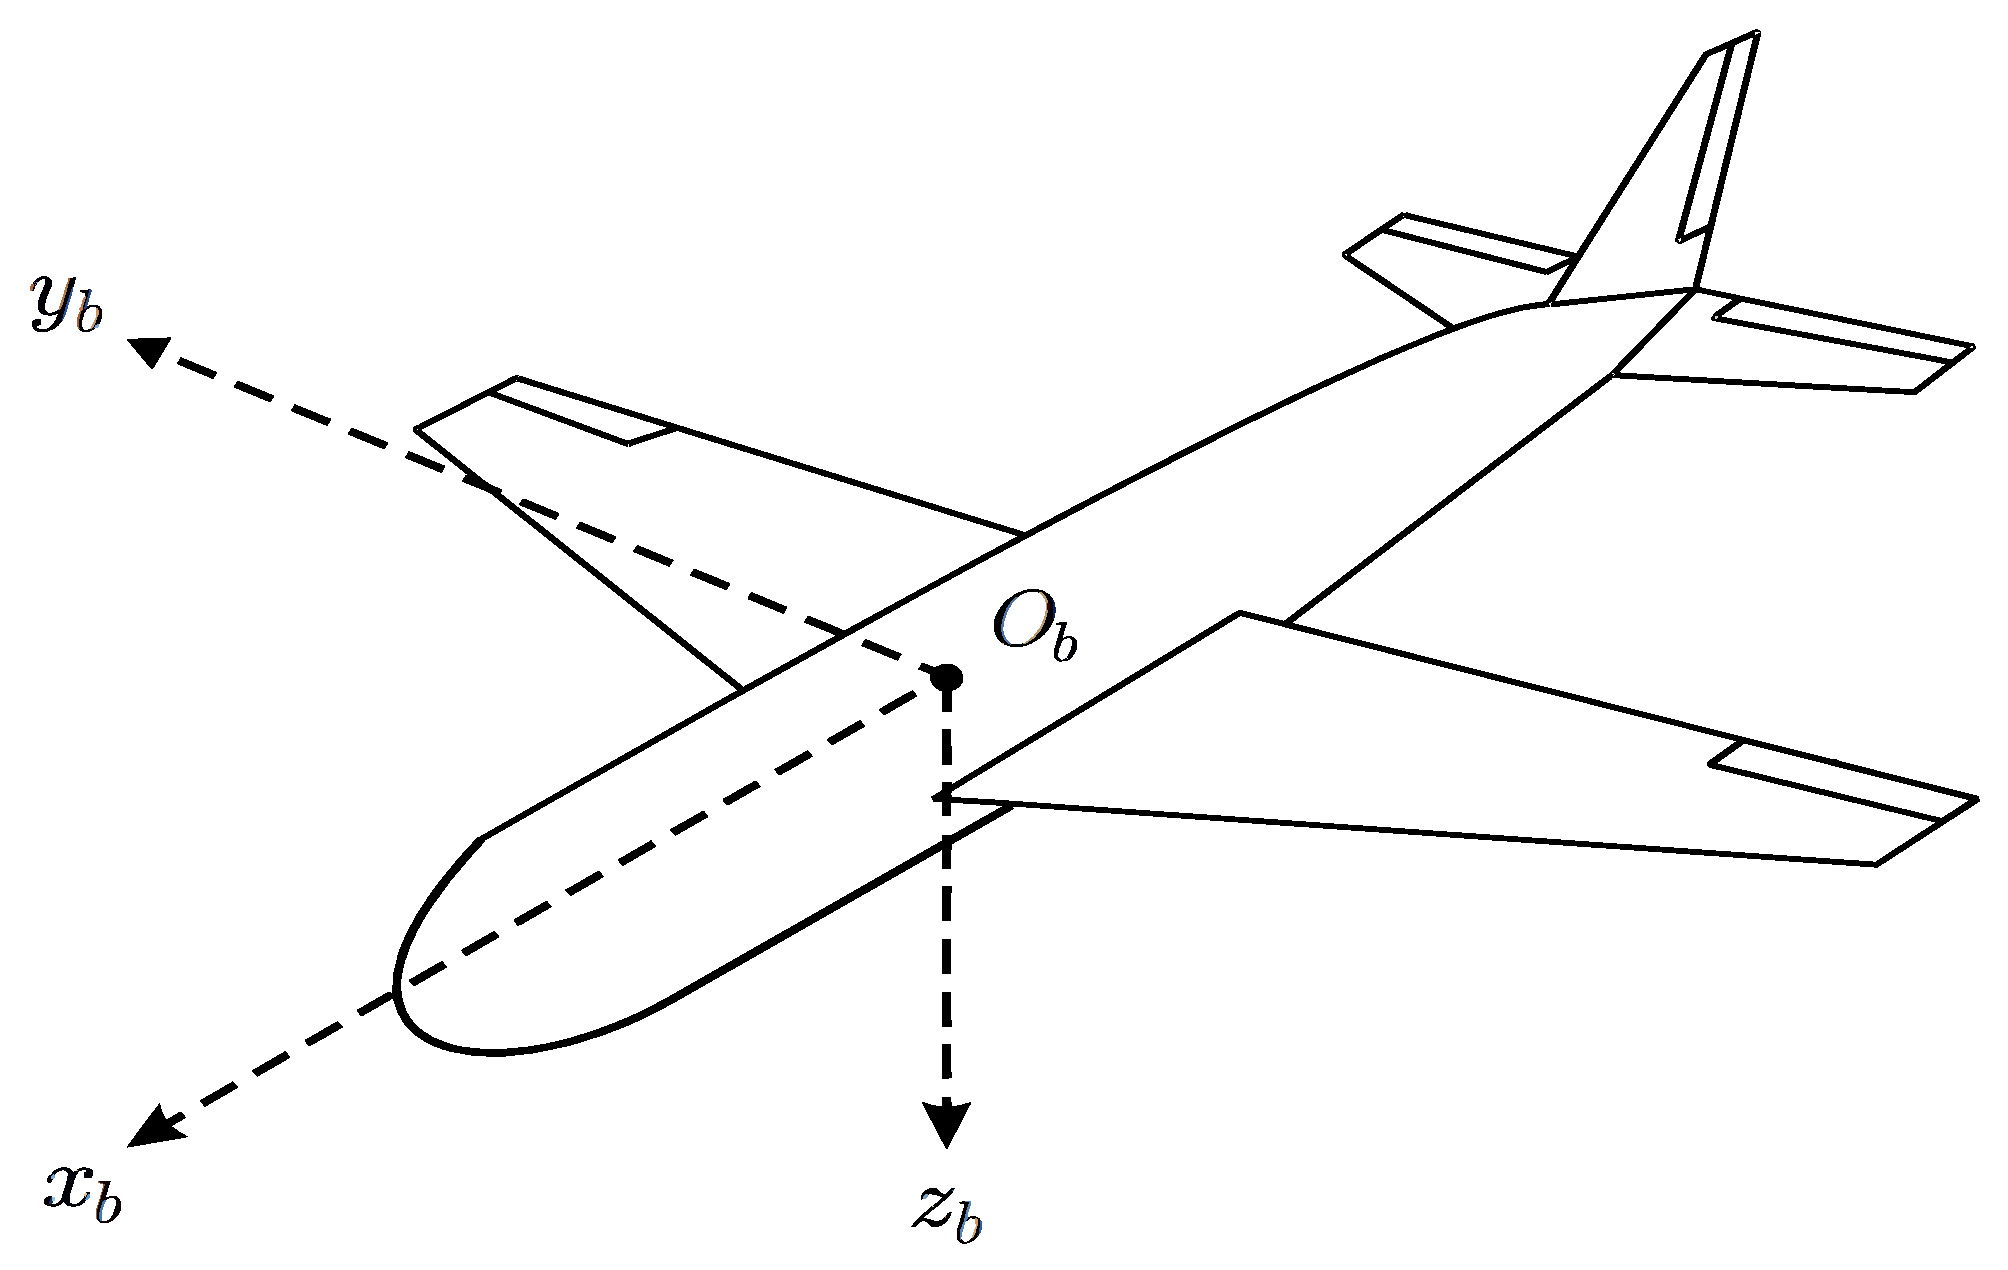
\includegraphics[width=0.50\textwidth]{aircraft_body_coordinate.pdf}
\caption{Aircraft Body Coordinate Frame}
%\label{fig:label}
\end{figure}

取无人机的重心位置为原点$o_b$,无人机左右对称的平面指向机头方向作为$o_b x_b$正方向,在左右对称平面内垂直于$o_b x_b$轴向下作为$o_b z_b$正方向,然后用右手定则确定$o_b y_b$正方向。
从无人机上方俯视时,$o_b y_b$正方向指向右侧机翼外侧。

\subsubsection{符号约定}

\paragraph{无参考系的单位向量}~

在没有参考系下,我们定义单位向量为:
\begin{equation}
e_1=[1,0,0]^T, e_2=[0,1,0]^T, e_3=[0,0,1]^T
\end{equation}

注意,三个坐标轴我们有时候用x,y,z表示,有时候用1,2,3表示,没有歧义时不加区分。

\paragraph{在EFCF下的的单位向量}~

在EFCF下沿EFCF三个坐标轴正方向的单位向量分别为:
\begin{equation}
{}^{e}e_1=e_1, {}^{e}e_2=e_2, {}^{e}e_3=e_3
\end{equation}

注意:${}^{e}e_1$表示$e_1$向量在EFCF坐标系下的值。

\paragraph{在ABCF下的的单位向量}~

在ABCF下沿ABCF三个坐标轴正方向的单位向量分别为:
\begin{equation}
{}^{b}b_1=e_1, {}^{b}b_2=e_2, {}^{b}b_3=e_3
\end{equation}

注意:${}^{b}b_1$表示$b_1$向量在ABCF坐标系下的值。

\paragraph{更通用的记号}~

我们在一个向量或矩阵的左下角或左上角做一些标记,来区分不同的坐标系。
通常,用$e$表示EFCF坐标系,用$b$表示ABCF坐标系。

对于向量,我们只在左上角做标记,表示该向量是相对于哪个坐标系而言。
比如,${}^{b}e_1$表示原本在EFCF中的向量$e_1$在ABCF中的值。

对于矩阵,尤其是当它被用于进行三维坐标变换时,我们用左下角的标记表示来源坐标系,左上角的标记表示目标坐标系。
比如,${}_{e}^{b}R$表示从EFCF变换到ABCF的矩阵$R$。

进一步,我们区分两种类型的三维旋转:
\begin{enumerate}
\item 向量的旋转。我们习惯性的用${}_{e}^{b}R$表示将一个向量从EFCF坐标系转换到ABCF坐标系。
\item 坐标系的旋转。我们习惯性的右上角增加一个撇号,用${}_{e}^{b}R^{'}$表示将EFCF坐标系转换到ABCF坐标系。
\end{enumerate}
注意,这两种类型是互逆的。

\subsection{欧拉角与姿态变换矩阵}

\subsubsection{定义欧拉角}

三次欧拉角旋转将飞机的ABCF与EFCF的方向连续关联。
\begin{figure}[H]%[htbp]
\centering
\includegraphics[width=0.80\textwidth]{euler_angles_and_frame_transformation.png}
\caption{Euler angles and frame transformation}
\label{euler_angles}
\end{figure}

\begin{figure}[H]%[htbp]
\centering
\includegraphics[width=0.80\textwidth]{euler_angles.png}
\caption{Frame transformation flow}
\label{frame_transformation}
\end{figure}

图\ref{euler_angles},\ref{frame_transformation}显示了欧拉角的定义,以及将坐标系EFCF变换到坐标系ABCF的过程。
我们记中间坐标系1为IF1,记中间坐标系2为IF2。
\begin{enumerate}
\item 首先给出EFCF,其三个坐标轴是$o_nx_n,o_ny_n,o_nz_n$;
\item 由EFCF绕$o_nz_n$轴正向旋转$\psi$角得到IF1(三个坐标轴是$o_1x_1,o_1y_1,o_1z_1$),该旋转角定义称为偏航角;
\item 由IF1绕$y_1$轴正向旋转$\theta$角被得到IF2(三个坐标轴是$o_2x_2,o_2y_2,o_2z_2$),该旋转角定义称为俯仰角;
\item 由IF2绕$x_2$轴正向旋转$\phi$角得到ABCF(三个坐标轴是$o_bx_b,o_by_b,o_bz_b$),该旋转角定义称为滚转角。
\end{enumerate}

\subsubsection{姿态变换矩阵}
姿态变换矩阵(也称旋转矩阵,也称方向余弦矩阵(Direction Cosine Matrix)),
可以将矢量和点坐标从ABCF转换到EFCF,反之也可以。

下面开始推导姿态变换矩阵,需要给出向量在EFCF中坐标到ABCF中坐标的变换关系。
注意:刚才定义的欧拉角是坐标系的旋转,但这里推导的是向量的旋转,有一定的区别。
为区分坐标轴还是向量,我们用大写字母表示坐标系和坐标轴,小写字母表示向量和坐标,并用下标表示不同坐标系。

\begin{enumerate}
\item 给定EFCF(三个坐标轴$O_nX_n,O_nY_n,O_nZ_n$),正向旋转$\psi$后得到IF1(三个坐标轴$O_1X_1,O_1Y_1,O_1Z_1$)。
假设在EFCF下有一个向量$o_nv_n=[x_n\quad y_n\quad z_n]^T$,向量$o_nv_n$在IF1下成为 $o_1v_1=[x_1\quad y_1\quad z_1]^T$。
它们之间的关系是:
\begin{equation}
\begin{bmatrix}x_1\\y_1\\z_1\end{bmatrix} = R_z(\psi)^{'}\begin{bmatrix}x_n\\y_n\\z_n\end{bmatrix},
\begin{bmatrix}x_n\\y_n\\z_n\end{bmatrix} = R_z(\psi)\begin{bmatrix}x_1\\y_1\\z_1\end{bmatrix}
\end{equation}
\item IF1正向旋转$\theta$后得到IF2(三个坐标轴$O_2X_2,O_2Y_2,O_2Z_2$),向量$o_1v_1$在IF2下成为$o_2v_2=[x_2\quad y_2\quad z_2]^T$。
它们之间的关系是:
\begin{equation}
\begin{bmatrix}x_2\\y_2\\z_2\end{bmatrix} = R_y(\theta)^{'}\begin{bmatrix}x_1\\y_1\\z_1\end{bmatrix},
\begin{bmatrix}x_1\\y_1\\z_1\end{bmatrix} = R_y(\theta)\begin{bmatrix}x_2\\y_2\\z_2\end{bmatrix}
\end{equation}
\item IF2正向旋转$\phi$后得到ABCF(三个坐标轴$O_bX_b,O_bY_b,O_bZ_b$),向量$o_2v_2$在IF2下成为$o_bv_b=[x_b\quad y_b\quad z_b]^T$。
它们之间的关系是:
\begin{equation}
\begin{bmatrix}x_b\\y_b\\z_b\end{bmatrix} = R_x(\phi)^{'}\begin{bmatrix}x_2\\y_2\\z_2\end{bmatrix},
\begin{bmatrix}x_2\\y_2\\z_2\end{bmatrix} = R_x(\phi)\begin{bmatrix}x_b\\y_b\\z_b\end{bmatrix}
\end{equation}
\item 将上述三个关系式串联起来,得到向量$o_nv_n$与向量$o_bv_b$的变换关系:
\begin{equation}
\begin{bmatrix}x_b\\y_b\\z_b\end{bmatrix} = R_x(\phi)^{'}R_y(\theta)^{'}R_z(\psi)^{'}\begin{bmatrix}x_n\\y_n\\z_n\end{bmatrix},
\begin{bmatrix}x_n\\y_n\\z_n\end{bmatrix} = R_z(\psi)R_y(\theta)R_x(\phi)\begin{bmatrix}x_b\\y_b\\z_b\end{bmatrix}
\end{equation}
\item 记欧拉角$\Theta$如下:
\begin{equation}
\Theta=\begin{bmatrix}\phi\\ \theta\\ \psi\end{bmatrix}
\end{equation}
\item 定义新的记号${R}_{e}^{b}(\Theta)$,表示将向量从EFCF旋转欧拉角$\Theta$到ABCF的变换矩阵。并作化简:
\begin{equation}
\begin{array}{rl}
	{R}_{e}^{b}(\Theta)&=R_x(\phi)^{'}R_y(\theta)^{'}R_z(\psi)^{'}\\
	~&= \begin{bmatrix}1 & 0 & 0\\0 & \cos\phi & \sin\phi\\0 & -\sin\phi & \cos\phi\end{bmatrix}
	\begin{bmatrix}\cos\theta & 0 & \sin\theta\\0 & 1 & 0\\-\sin\theta & 0 & \cos\theta\end{bmatrix}
	\begin{bmatrix}\cos\psi & \sin\psi & 1\\-\sin\psi & \cos\psi & 1\\0 & 0 & 1\end{bmatrix}\vspace{1ex} \\
	~&= \begin{bmatrix}
		\cos\theta\cos\psi & \cos\theta\sin\psi & \sin\theta\\
		-\cos\phi\sin\psi - \sin\phi\sin\theta\cos\psi & 
			\cos\phi\cos\psi - \sin\phi\sin\theta\sin\psi & 
			\sin\phi\cos\theta\\
		\sin\phi\sin\psi - \cos\phi\sin\theta\cos\psi & 
			-\sin\phi\cos\psi - \cos\phi\sin\theta\sin\psi & 
			\cos\phi\cos\theta	
	\end{bmatrix}
\end{array}
\end{equation}
\item 定义新的记号${R}_{b}^{e}(\Theta)$,表示将向量从ABCF旋转欧拉角$\Theta$到EFCF的变换矩阵。并作化简:
\begin{equation}
\begin{array}{rl}
	{R}_{b}^{e}(\Theta)&=R_z(\psi)R_y(\theta)R_x(\phi)\\
	~&= \begin{bmatrix}\cos\psi & -\sin\psi & 1\\ \sin\psi & \cos\psi & 1\\0 & 0 & 1\end{bmatrix}
	\begin{bmatrix}\cos\theta & 0 & -\sin\theta\\0 & 1 & 0\\ \sin\theta & 0 & \cos\theta\end{bmatrix}
	\begin{bmatrix}1 & 0 & 0\\0 & \cos\phi & -\sin\phi\\0 & \sin\phi & \cos\phi\end{bmatrix}\vspace{1ex} \\
	~&= \begin{bmatrix}
		\cos\theta\cos\psi &
		-\sin\phi\cos\psi - \cos\phi\sin\theta\sin\psi &
		\sin\phi\sin\psi - \cos\phi\sin\theta\cos\psi \\
		\cos\theta\sin\psi &
		\cos\phi\cos\psi - \sin\phi\sin\theta\sin\psi &
		-\cos\phi\sin\psi - \sin\phi\sin\theta\cos\psi \\
		\sin\theta &
		\sin\phi\cos\theta &
		\cos\phi\cos\theta	
	\end{bmatrix}
\end{array}
\end{equation}
\end{enumerate}


\section{四元数}

Quaternions were ``invented'' by Hamilton in 1843. 
From their very inception, they was meant to represent, in an unified form, both scalar and vector quantities.



值得一提的是:
1. 四元数的实现,使用了Module概念,可以支持Nat、Z、Real等不同类型的四元数。
2. 证明了四元数乘法公式。

无人机的姿态表示,最常见的有三种模型。
它们是欧拉角、旋转矩阵、四元数,这些模型之间可以相互转换。
这些不同的模型各有利弊,主要的区别如下:
(a). 欧拉角:直观,但有奇异性,需要处理特殊情况。
(b). 旋转矩阵:是欧拉角和四元素的一个过渡。
(c). 四元数:计算量小,没有奇异性,但不太直观。
这些模型需要配合使用,以便计算量小而且直观,从而实现满足用户需求的高效算法。

%我们在研究飞行姿态问题时就发现了多个出版物中的歧义表述、公式错误。例如:
%\begin{enumerate}
%\item \cite{qq} p91, 欧拉角的正负规定,有歧义
%\item \cite{qq} p92,由图5.5中欧拉角的定义到公式5.3,第一个和第三个矩阵都有错误。
%\item \cite{qq} p94,公式5.12中当theta=-pi/2时,a13,a23漏了一个负号。不过前提是其依赖的公式5.9是正确的。而不幸的是该公式也是错误的,因为之前的公式5.3是错误的。
%\item \cite{cm} p153,公式4.33,4.44,4.45合成公式4.46,要么有一个输入是错误的,要么推导过程是错误的,总之前后矛盾。
%\end{enumerate}



\begin{thebibliography}{99}
\bibitem{qq} Quan Q. Introduction to multicopter design and control. Springer, 2017.
\bibitem{cm} Goldstein H, Poole C, Safko J. Classical Mechanics (Third Edition). Addison-Welsley, San Francisco, 2001.
\bibitem{fcs} Ducard G J. Fault-tolerant flight control and guidance systems: practical methods for small unmanned aerial vehicles. Springer-Verlag, Longdon, 2009.
\bibitem{mathForCS} Ernest Davis. Linear Algebra and Probability for Computer Science Applications. Taylor \& Francis Group, LLC 2012.
\end{thebibliography}

\end{document}